% Free range VHDL
% Authors: Bryan Mealy, Fabrizio Tappero
% Date: May, 2011
%
% (C) 2011 B. Mealy, F. Tappero
%
% !TEX root = master.tex
%
\chapter{Registers and Register Transfer Level}
The concept of a register in VHDL and its subsequent use in digital circuit design is probably one of the more straightforward concepts in VHDL. A register in VHDL is simply a vector version of a D flip-flop in which all operations on the flip-flops occur simultaneously. The ``register transfer level'', or RTL, is a flavor of design that is primarily concerned with how and when data is transferred between the various registers in a digital system. RTL-level design in often associated with "data-path" designs which require the careful control and timing of the data that is being transferred between registers. The controls associated with even simple registers are sufficient to ensure that some outside entity has adequate control over the "sequencing" of data through the circuit associated with the data-path. In these cases, the proper sequencing of data transfers is controlled by a FSM. 

The study of RTL-level design is best accomplished in the context of a data-path design. The design of data-paths is best accomplished in the context of a digital circuit that has some purpose such as an arithmetic logic unit design. Both of these topics are beyond what needs to be mentioned here. The good news is that the simplicity of the registers makes for a quick introduction to the matter. Major circuit implementations are saved for some other time.

\begin{leftbar}
\begin{minipage}[t]{0.52\textwidth}
\vspace{10pt}
\noindent
\textbf{EXAMPLE 23.}
Use VHDL behavioral modeling to design the 8-bit register that has a synchronous active high parallel load signal LD. Consider the load of the register to be synchronized to rising edges of the clock. 
\end{minipage}
\begin{minipage}[t]{0.47\textwidth}
\vspace{0pt}\raggedright
    \centering
	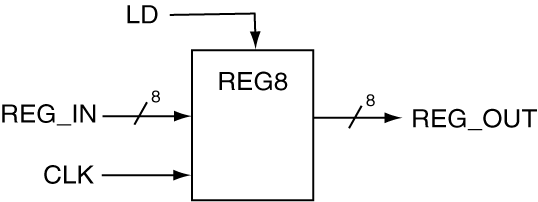
\includegraphics[width=5.2cm]{r_rtl/ex23.png}
\end{minipage}
\end{leftbar}
\noindent
\textbf{SOLUTION.} The solution for the 8-bit register looks amazingly similar to a model of a D flip-flop. The full solution to Example 23 is shown in Listing \ref{ex23_code}. As usual, there are a couple of things worth noting in this solution.
\begin{my_list}
\item Note that there is an \texttt{if} statement that does not contain a corresponding \texttt{else} which is what generates the memory element. For this example, there are considered to be eight bit-sized memory elements (flip-flops). For this example the flip flops are considered to be D-type flip-flops. The storage elements are associated with the \texttt{REG\_OUT} bundle. The ease in using VHDL code to generate D flip-flops in this manner makes D flip-flops the most widely used type of flip-flop in digital design.

\item The code uses a bundle signal for both the input and output. The assignment of the bundles to other bundles is straightforward in VHDL as is shown in the code. In many cases, such as the one in this example, there is no need to use a bundle access operator in the VHDL model. 

\item The assignment of the input to the output is based on characteristics of both the clock edge and the state of the LD signal. The approach taken in the VHDL model shown in Listing \ref{ex23_code} is to provide a separate \texttt{if} clause for both the LD and CLK signals. Only one \texttt{if} statement could have been used by making both conditions associated with the single \texttt{if} clause but this is not considered good VHDL programming practice when dealing with synchronized elements. In other words, you should always strive to keep special conditions associated with the clocking signal separate from all other conditions associated with the action in question. Clock signals are somewhat special in the VHDL land; you should get into the habit of treating them gently. 

\item Since signals \texttt{REG\_IN} and \texttt{LD} are required to be synchronous they do not appear inside the process sensitivity list.
\end{my_list}

\noindent
\begin{minipage}{0.99\linewidth}
\begin{lstlisting}[label=ex23_code, caption=Solution to Example 23.]
-- library declaration
library IEEE;
use IEEE.std_logic_1164.all;
-- entity
entity reg8 is
    Port ( REG_IN  :  in std_logic_vector(7 downto 0);
           LD,CLK  :  in std_logic;
           REG_OUT : out std_logic_vector(7 downto 0));
end reg8;
-- architecture
architecture reg8 of reg8 is
begin
   reg: process(CLK)
   begin
      if (rising_edge(CLK)) then 
         if (LD = '1') then 
            REG_OUT <= REG_IN; 
         end if;
      end if;
   end process; 
end reg8;
\end{lstlisting}
\end{minipage}

The circuit in the following example is slightly more complex than most of the examples seen so far. Additionally, remember that there are many different solutions to the same problem. This is a common occurrence in VHDL; in fact, many times there is no best method for implementing a given circuit. The following examples are essentially the same problem solved using two different but functionally equivalent solutions.

\begin{leftbar}
\begin{minipage}[t]{0.5\textwidth}
\vspace{10pt}
\noindent
\textbf{EXAMPLE 24.}
Use VHDL behavioral modeling to design the circuit shown on the right. Consider both the loading signals to be active high. Consider the circuit to be synchronized to the rising edge of the clock signal. 
\end{minipage}
\begin{minipage}[t]{0.5\textwidth}
\vspace{0pt}\raggedright
    \centering
	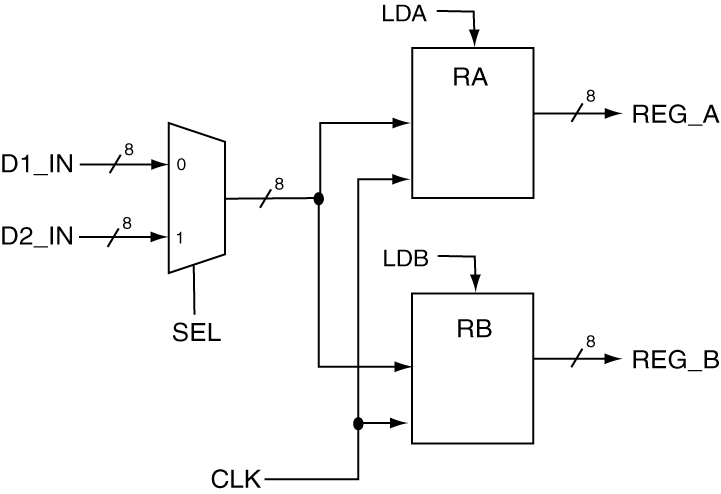
\includegraphics[width=5.7cm]{r_rtl/ex24.png}
\end{minipage}
\end{leftbar}
\noindent
\textbf{SOLUTION.} The circuit shown in Example 24 includes two 8-bit registers and a 2:1 MUX. This is an example of a bus-based data transfer in the output of the MUX that is connected to the inputs of the two registers. Each of the two registers has its own independent load control input. The solution to Example 24 is shown in Listing \ref{ex23_code}. And as we have grown to expect, there are a couple of things worth noting about this solution. 
\begin{my_list}
\item There are three concurrent statements in this solution: two behavioral models and one data-flow model. 

\item There is a separate process for each of the two registers. Although it would have been possible to represent both registers using one process, it would have been somewhat complicated and somewhat hard to understand. The better approach in VHDL is always to break tasks down into their logically separate functions and use the various VHDL modeling techniques as tools to keep the tasks separate and simple. The reality is that the synthesizer becomes your friend if you provide it with simple models. The quantity of VHDL code describing a certain design is immaterial; the complexity of any given model is determined by the most complex piece of code in the model. Simple is always better in VHDL.

\item All of signals shown in the Example 24 have external linkage except for the output of the MUX. The MUX output is connected to the inputs of both registers. The final approach taken in this solution is typical in VHDL: many processes that communicate with each other through shared signals. In this example, there is only one shared signal but this is a fairly simple program. The same inter-process communication model is used in more complicated circuits.

\item The model for the 2:1 MUX uses the terminology \texttt{(others => '0')}. This is a short-hand terminology for assigning all of the outputs to '0'. The real nice part about this instruction is that you do not need to know how many 0’s you need to write. This is a nice feature in that if the width of the associated bundle were to change, this particular line of code would not need to be modified. 
\end{my_list}

\noindent
\begin{minipage}{0.99\linewidth}
\begin{lstlisting}[label=ex24_code, caption=Solution to Example 24.]
-- library declaration
library IEEE;
use IEEE.std_logic_1164.all;
-- entity
entity ckt_rtl is
   port (D1_IN,D2_IN : in  std_logic_vector(7 downto 0);
             CLK,SEL : in  std_logic; 
             LDA,LDB : in  std_logic; 
         REG_A,REG_B : out std_logic_vector(7 downto 0)); 
end ckt_rtl; 
-- architecture
architecture rtl_behavioral of ckt_rtl is 
   -- intermediate signal declaration ---------------
   signal s_mux_result : std_logic_vector(7 downto 0);
begin

   ra: process(CLK) -- process
   begin
      if (rising_edge(CLK)) then 
         if (LDA = '1') then 
            REG_A <= s_mux_result; 
         end if;
      end if;
   end process; 
	
   rb: process(CLK) -- process
   begin
      if (rising_edge(CLK)) then 
         if (LDB = '1') then 
            REG_B <= s_mux_result; 
         end if;
      end if;
   end process; 
	
   with SEL select
   s_mux_result <= D1_IN when '1', 
                   D2_IN when '0', 
                   (others => '0') when others; 
end rtl_behavioral;
\end{lstlisting}
\end{minipage}

\begin{leftbar}
\begin{minipage}[t]{0.5\textwidth}
\vspace{10pt}
\noindent
\textbf{EXAMPLE 25.}
Use VHDL structural modeling to design the circuit shown on the right. Consider both of the loading signals to be active high. Consider the circuit to be synchronized to the rising edge of the clock signal.
\end{minipage}
\begin{minipage}[t]{0.5\textwidth}
\vspace{0pt}\raggedright
    \centering
	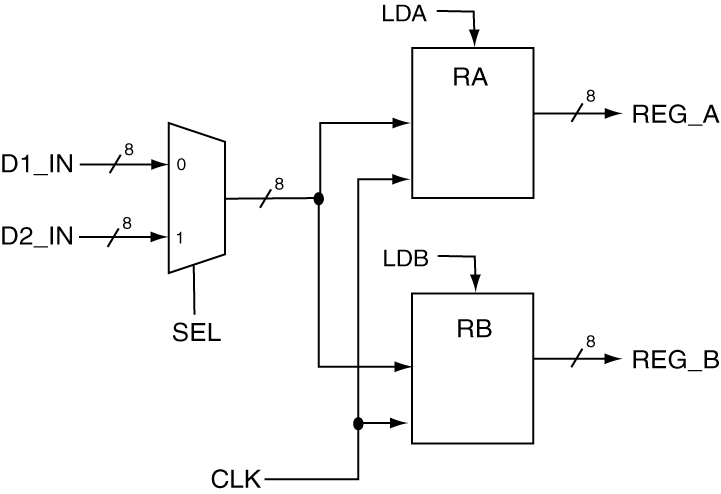
\includegraphics[width=5.7cm]{r_rtl/ex25.png}
\end{minipage}
\end{leftbar}
\noindent
\textbf{SOLUTION.} The solution to Example 25 is shown in Listing \ref{ex25_code}. There is not too much interesting to note here. This is a more realistic example of a structural model compared to the example presented in the section on structural modeling. There are only a few new and wonderful things to note about this solution.

\begin{my_list}
\item The very important thing to note about the solution in Listing \ref{ex25_code} is to not be intimidated by the sheer quantity of code listed. The code is well structured; if you are able to recognize this structure, you will be more apt to understand the solution. And better yet, you will be more on your way to being able to write your own amazing chunks of VHDL code. 

\item The VHDL source code shown in Listing \ref{ex25_code} is nicely formatted. In particular, the code is nicely indented. Properly indented code is highly desirable in that it nicely presents information based on the indentation. No surprise here but properly formatted code is easier to understand. Better yet, good looking code leads people who may or may not know otherwise into thinking your code is as actually as good as it looks. In this busy world of ours, a quick glance is just about all the time people (bosses and teachers) have to dedicate to perusing your VHDL source code.
\end{my_list}

\noindent
\begin{minipage}{0.99\linewidth}
\begin{lstlisting}[label=ex25_code, caption=Solution to Example 25 using a structural modeling approach.]
entity mux2t1 is                                    --- ENTITY
   port (  A,B : in  std_logic_vector(7 downto 0); 
           SEL : in  std_logic; 
         M_OUT : out std_logic_vector(7 downto 0)); 
end mux2t1; 
architecture my_mux of mux2t1 is                    --- ARCHITECTURE
begin 
   with SEL select
   M_OUT <= A when '1', 
            B when '0', 
            (others => '0') when others; 
end my_mux;
entity reg8 is                                      --- ENTITY
    Port (  REG_IN : in  std_logic_vector(7 downto 0);
            LD,CLK : in  std_logic;
           REG_OUT : out std_logic_vector(7 downto 0));
end reg8;
architecture reg8 of reg8 is                       --- ARCHITECTURE
begin
   reg: process(CLK)
   begin
      if (rising_edge(CLK)) then 
         if (LD = '1') then 
            REG_OUT <= REG_IN; 
         end if;
      end if;
   end process; 
end reg8;
entity ckt_rtl is                                    --- ENTITY
   port (D1_IN,D2_IN : in  std_logic_vector(7 downto 0);
             CLK,SEL : in  std_logic; 
             LDA,LDB : in  std_logic; 
         REG_A,REG_B : out std_logic_vector(7 downto 0)); 
end ckt_rtl; 
architecture rtl_structural of ckt_rtl is           --- ARCHITECTURE
   -- component declaration
   component mux2t1 
      port (  A,B : in  std_logic_vector(7 downto 0); 
              SEL : in  std_logic; 
            M_OUT : out std_logic_vector(7 downto 0)); 
   end component;
   component reg8 
       Port (  REG_IN : in  std_logic_vector(7 downto 0);
               LD,CLK : in  std_logic;
              REG_OUT : out std_logic_vector(7 downto 0));
   end component;
   -- intermediate signal declaration
   signal s_mux_result : std_logic_vector(7 downto 0); 	
begin
   ra: reg8
   port map ( REG_IN => s_mux_result,
                  LD => LDA,
                 CLK => CLK,
             REG_OUT => REG_A ); 
   rb: reg8
   port map ( REG_IN => s_mux_result,
                  LD => LDB,
                 CLK => CLK,
             REG_OUT => REG_B ); 			 
   m1: mux2t1
   port map (   A => D1_IN, 
                B => D2_IN,
              SEL => SEL,
            M_OUT => s_mux_result); 				 
end rtl_structural;
\end{lstlisting}
\end{minipage}

\section{Important Points}

\begin{my_list}
\item VHDL can be used to easily implement circuits at the register transfer level. The corresponding VHDL models can be implemented in either structural of full behavioral format. 

\item RTL level VHDL models should strive for simplicity in their designs. If the behavioral models in the RTL design become complicated, the chances that your circuit works correctly greatly diminish due to the synthesis of the complicated circuit. 
\end{my_list}




